\documentclass{report}

\usepackage{graphicx}

\title{Simple Regression Analysis of Advertising Data}

\author{Alexander Lee}

\date{\today}

\usepackage{Sweave}
\begin{document}
\Sconcordance{concordance:lab09.tex:lab09.Rnw:%
1 10 1 1 0 13 1 1 2 1 0 1 1 12 0 1 2 13 1 1 2 6 0 1 1 22 0 1 2 14 1}

\maketitle

\begin{abstract}
This report seeks to replicate the research found in \emph{Simple Linear Regression}, chapter 3 of the book \emph{An Introduction to Statistical Learning} by Gareth James, et al., on a set of advertising data.
\end{abstract}

\section*{Introduction}
The goal of this research is to use existing data to formulate a marketing plan that will result in higher product sales. To that end, we will run a linear regression to model the increase of sales against the amount of money spent on marketing the product. We will analyze this to determine how advertising affects sales, and how the company should budget for advertising in order to increase sales of the product.

\section*{Data}
The Advertising data set consists of the $Sales$ (in thousands of units) of a particular product in 200 different markets, along with advertising budgets (in thousands of dollars) for the product in each of those markets for three different media: $TV$, $Radio$, and $Newspaper$. We work primarily with the $TV$ data for this project, observing the effects of different levels of budget for TV advertising on the sales of units.

\begin{Schunk}
\begin{Sinput}
> load('regression.RData')
> head(advertising)
\end{Sinput}
\begin{Soutput}
  X    TV Radio Newspaper Sales
1 1 230.1  37.8      69.2  22.1
2 2  44.5  39.3      45.1  10.4
3 3  17.2  45.9      69.3   9.3
4 4 151.5  41.3      58.5  18.5
5 5 180.8  10.8      58.4  12.9
6 6   8.7  48.9      75.0   7.2
\end{Soutput}
\end{Schunk}

\section*{Methodology}
We look at the relationship between $Sales$ and $TV$ budget using a simple linear model:


  $Sales = \alpha + \beta * TV$


That is, we predict there to be a linear relationship between the amount of money spent on TV advertising and the number of sales of units. We approximate $\alpha$ and $\beta$ using a linear regression under the least squares criterion.


\section*{Results}
We computed the correlation coefficients using the $lm$ function, with $TV$ as a function of $Sales$.

\begin{Schunk}
\begin{Sinput}
> print('Table 1: Information about the Linear Regression')
\end{Sinput}
\begin{Soutput}
[1] "Table 1: Information about the Linear Regression"
\end{Soutput}
\begin{Sinput}
> ad_summ
\end{Sinput}
\begin{Soutput}
Call:
lm(formula = Sales ~ TV, data = advertising)

Residuals:
    Min      1Q  Median      3Q     Max 
-8.3860 -1.9545 -0.1913  2.0671  7.2124 

Coefficients:
            Estimate Std. Error t value Pr(>|t|)    
(Intercept) 7.032594   0.457843   15.36   <2e-16 ***
TV          0.047537   0.002691   17.67   <2e-16 ***
---
Signif. codes:  0 '***' 0.001 '**' 0.01 '*' 0.05 '.' 0.1 ' ' 1

Residual standard error: 3.259 on 198 degrees of freedom
Multiple R-squared:  0.6119,	Adjusted R-squared:  0.6099 
F-statistic: 312.1 on 1 and 198 DF,  p-value: < 2.2e-16
\end{Soutput}
\end{Schunk}

The estimates of these coefficients, $\alpha$ and $\beta$, are 7.0326 and 0.0475, respectively; that is, for every \$1,000 increase in spending
on TV advertising, sales are projected to increase by 48 units. On average, data will deviate from the true regression model by 3.2587. An $R^2$ of 0.6119, means 61.19\% of the variability is explained by the model. An F-statistic of 312.145 means that the coefficients found by our model are very likely to be close to the true regression values.

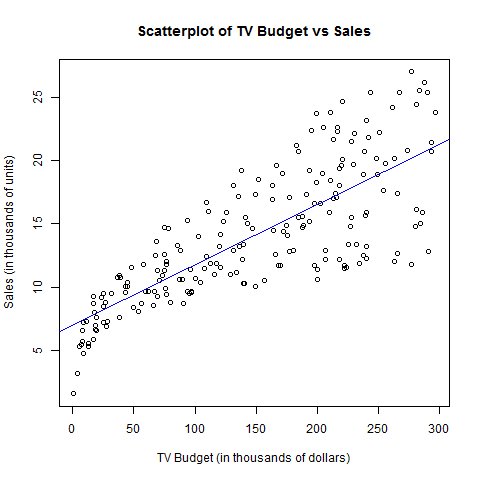
\includegraphics{scatterplot-tv-sales.png}


\section*{Conclusion}
There is a positive correlation between the budget for TV advertising and Sales; however, this relationship is very minimal. For every \$1,000 spent on advertising only another 48 units are sold, so each unit would have to
cost at least 21.04 in order to break even or profit off the units sold. 


\end{document}


